
\chapter{Concept}\label{CH3}

%\section{X-band sensor description and interface analysis}
\section{X-band silicon sensor serial data acquisition}
\section{Sensor control}
\section{Firmware}
\section{Communication interfaces}

%\subsection{Deserialisation using CMOS CMV4000}
%\subsection{Programmable sequencer}
%
%\section{Firmware implementation}
%\subsection{Operating system architecture}
%\subsection{Software digital system control}
%
%\section{Synchronisation}
%\subsection{IEEE1588}
%\subsection{External trigger}
%
%\section{Interfaces}
%\subsection{1 GbE Ethernet}
%\subsection{Serial ATA}
%
%\section{Hardware tests}

%\section{Development platform}
%    \subsection{Xilinx Zynq SoC}
%    \subsection{Development board ZC706}
%
%\section{Design of framework camera subsystems}
%    \subsection{Data transfer}
%        \subsubsection{1 Gigabit Ethernet}
%
%        The 1 Gigabit Ethernet interface (1000BASE-X\cite{WWW:ETH_1000BASEX}, or 802.3z) is a network data transfer
%        interface. Xilinx Zynq SoC provides two possible ways of adding a support of 1 GbE, in programmable logic or using
%        build-in hardware MAC\footnote{Media Access Control\cite{WWW:MAC}}. 
%
%        Table \ref{tab:1gbe_pros_cons} presents a comparison between the two possible implementations.  
%
%
%        \begin{table}
%            \centering
%            \caption{Pros and cons of different 1 GbE implementations}
%            %\begin{tabular}{|p{3cm}||p{5cm}|p{5cm}|}
%            \begin{tabularx}{\textwidth}{|l|X|X|}
%                \hline
%                & \textbf{1 GbE with PHY}  & \textbf{1 GbE in programmable logic}  \\ 
%                \hline
%                \hline
%                \textbf{Pros}    & 
%                \vspace{0.1cm}
%                \begin{itemize}
%                    \item more reliable  
%                    \item shorter development time
%                \end{itemize}
%
%                & 
%
%                \vspace{0.1cm}
%                \begin{itemize}
%                    \item lower cost 
%                    \item more versatile 
%                \end{itemize}
%                \\  
%                \hline
%                \textbf{Cons}    &  
%
%
%                \vspace{0.1cm}
%                \begin{itemize}
%                    \item high cost (PHY chip)
%                    \item limited future upgrades 
%                \end{itemize}
%
%                & 
%                \vspace{0.1cm}
%                \begin{itemize}
%                    \item longer development time 
%                    \item less reliable  
%                \end{itemize}
%
%                \\  
%                \hline
%            \end{tabularx}
%            \label{tab:1gbe_pros_cons}
%        \end{table}
%
%        The most important aspect of the development of 1 GbE is the usefulness in scientific camera systems. From the two
%        solutions the implementation of 1 GbE using programmable logic is a better solution, because it's more versatile.  
%
%%
%%\textbf{Pros:}
%%\begin{itemize}
%%    \item No need to use PHY chip in the camera hardware (lower cost)
%%    \item Possibility to upgrade the IP Core to the 10 Gbit version in future
%%    \item Full support by Zynq SoC ~\cite{XIL:PCS_PMA}
%%    \item PTP support  
%%\end{itemize}
%%
%%
%%\textbf{Cons:}
%%\begin{itemize}
%%    \item More complicated development
%%    \item Performance is dependent on the PCS/PMA Linux driver quality
%%    \item Not supported by FreeRTOS and Baremetal code on Zynq SoC 
%%    \item Necessity of using 1 GbE SFP transceiver (additional cost)
%%\end{itemize}
%%
%%As for the camera framework, the pros far outweighs the cons. The increased complexity allows for the future improvement
%%of the whole system.   
%%
%    \subsection{Operating system architecture}
%    \subsection{Video data acquisition from the sensor}
%    \subsection{Software based digital system control}
%    \subsection{Multicamera synchronisation}
%
%In this chapter, the concept of a camera design framework is presented. Based on the requirement analysis made in Chapter 2.
%Firstly, main camera functions are listed and defined. In this chapter, the \emph{key project decisions} are made.
%For an embedded system design, some irreversible decisions have to be made at the beginning of the design, such as:
%choosing an architecture of the Main Processing Unit, sensor type, operating system etc. These reflect on the future fulfilment of the 
%requirements. 
%
%%Due to complexity of the project many members of PERG\footnote{Photonics and Web Engineering Group} were involved in the
%%process of development of the camera framework. It is clearly stated in this and following sections which parts were
%%developed by whom.  
%
%%Section~\ref{ch2:methodology} contains general information about the design methodology for the embedded system
%%engineering design, which aims to present a view on the way the project was being worked on.  
%
%\section{Design idea}\label{ch3:ida}
%
%The purpose of this project is to design a framework that allows for testing and verification of any scientific or
%task-specialised camera system. The project was designed with a bottom-up methodology in mind, taking into account how
%a typical camera design process would look like. To provide versatility of the solutions there are many features options 
%for the designer to choose from depending on the needs. 
%
%The basic idea is to have a common architecture where main design blocks can be changed or adjusted. The main component of the camera
%framework is the Main Processing Unit (MPU) which consists of programmable logic and a general purpose processor. 
%Any given sensor can be connected to the MPU either directly to the programmable logic or using a dedicated analog
%front-end (AFE), as in the case of CCD sensors. The data coming from the sensor can be processed in the programmable
%logic or in the general purpose processor. Storage can be made on a non-volatile medium or transmitted directly to the PC or
%any other device. The operating system of the camera can be changed depending on the needs and any additional sensor or
%actuator control can be implemented. 
%
%Having the basic blocks working minimizes the amount of work needed for the developer to make a prototype work. The
%The figure~\ref{FIG:BASIC_BLOCK_DIAG} presents the basic block diagram. Each of these components is defined in this 
%section and some main project decisions are made which have to be done at an early stage of development of any embedded system. 
%\begin{figure}[h!]
%    \centering
%    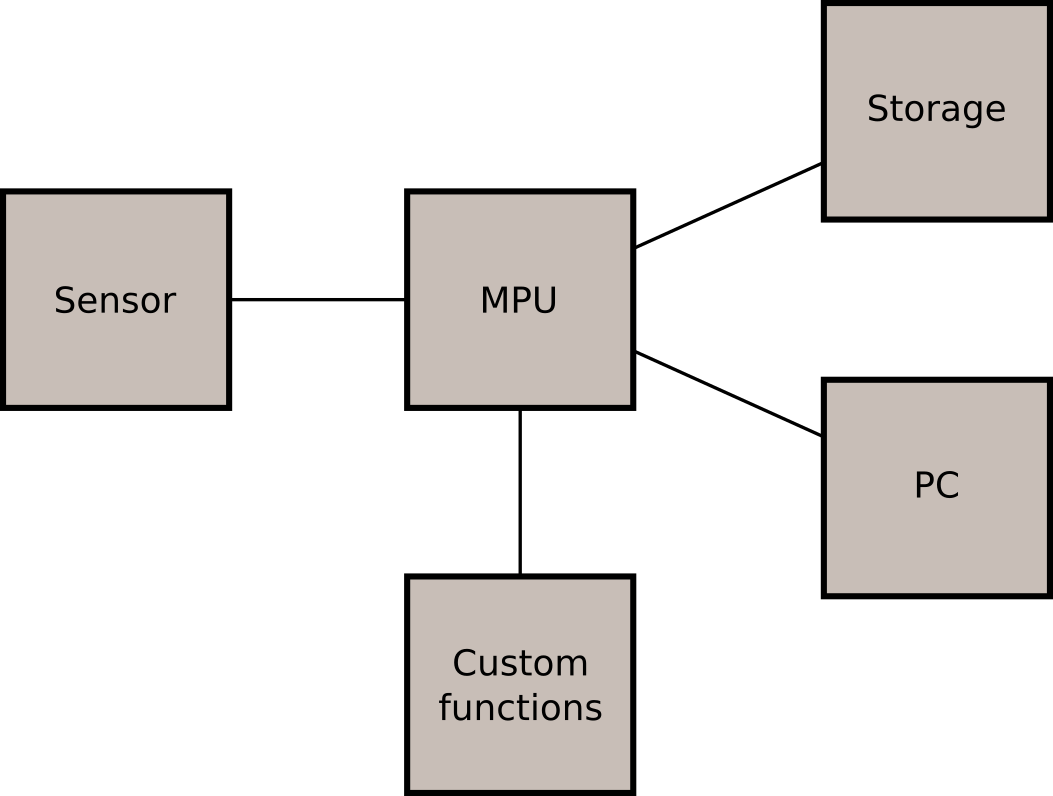
\includegraphics[width=12cm]{img/concept/block_diagram_basic.png}
%    \caption{Basic diagram of Camera Framework}
%    \label{FIG:BASIC_BLOCK_DIAG}
%\end{figure} 
%
%
%\section{Main project decisions}~\label{ch3:decisions}
%
%After the analysis of requirements key project decisions have been made. The main decisions were to define and
%characterise a Main Processing Unit, sensor and the interfaces that were to be used in the project.    
%
%\subsection{Main processing unit}
%
%An MPU\footnote{Main Processing Unit} for a camera consists of:
%
%\begin{itemize}
%    \item Camera interface 
%    \item High speed interface for data transmission 
%    \item Can run Embedded Linux and an RTOS
%\end{itemize}
%
%The requirement analysis (\ref{ch2:req_analysis}) suggests that an FPGA can be used as an MPU. 
%This is due to the fact that FPGAs allow for connecting any desired sensor to the camera. This might not always be done directly, 
%since in certain cases 
%(such as a CCD sensor) a specialised AFE and readout electronics have to be designed. Nevertheless, FPGAs are 
%versatile devices for this kind of application. They can also be used for video processing. The architecture allows for
%efficient video processing, which can process the video data in real-time. One of the real-world application of FPGAs in
%camera systems are ADAS\footnote{Advanced driver assistance systems} where they are used for radar and image processing
%\cite{PAPER:UAV_CAMERA,PAPER:DYN_RECONF_CAMERA,PAPER:ADAS}.
%
%The requirement of versatility of camera framework in terms of supporting different sensors (hardware requirement) and
%possibility to run a high level operating system (software requirement) leaves the following development paths for
%choosing the Main Processing Unit:
%
%\begin{enumerate}[nolistsep]
%    \item use two ICs: an  FPGA and an Application Processing Unit
%    \item use just an FPGA with soft processor done in logic   
%    \item use an SoC with FPGA and APU on one silicon die 
%\end{enumerate}
%
%The table~\ref{tab:ic_comp} presents the pros and cons of each scenario with examples of possible devices that can be used.
%
%% \begin{table}
%%   \centering
%%   \caption{Comparision of possible scenarios of choosing an MPU}
%%   \begin{tabular}{l|c|c|c|}
%%     \hline
%%     \textbf{Characteristic} & FPGA + MPU & FPGA with softprocessor & SoC (FPGA + APU) \\ 
%%     \textbf{Pros} & 
%%     Design is easily dividable. 
%%     Discrete MPU can have the highest clock speed. 
%%     An FPGA can act as glue logic for a sensor interface.
%%         & 
%%     Single IC solution. 
%%     Softprocessor is capable of running an OS like Linux or FreeRTOS\@.
%%     Softprocessor has direct access to FPGA internal bus (AHB/AXI).  
%%         &  
%%     APU is capable of running an OS like Linux or FreeRTOS\@.
%%     Hardened processor has higher clock speed than a softprocessor and comparable to a discrete MPU. \\
%%     APU has direct access to FPGA internal bus (AHB/AXI).  
%%     \hline
%%     \textbf{Cons} & 
%%     Troublesome interfacing between FPGA and MPU. 
%%     & 
%%      Softprocessor can run only on low frequencies~\ref{data:microblaze}.
%%      Interrupt-latency is higher than in SoC~\ref{art:softprocessor_rtos}.  
%%     &
%%      Cost is higher than FPGA-only solution. 
%%      \\ 
%%     \hline
%%   \end{tabular}
%%   \label{tab:ic_comp}
%% \end{table}
%% 
%
%\begin{table}
%    %    \centering
%    \caption{Comparison of possible scenarios of choosing an MPU}
%    \begin{tabularx}{\textwidth}{|c|X|X|}
%        \hline
%         &  \textbf{Pros:}   &  \textbf{Cons:} \\
%        \hline
%        \hline
%        \textbf{FPGA+AP\footnote{Application Processor}} & 
%        \vspace{0.1cm}
%        \begin{itemize}
%            \item  Discrete MPU can have the highest clock speed. 
%            \item  An FPGA can act as glue logic for a sensor interface.
%        \end{itemize}
%        &
%        \vspace{0.1cm}
%        \begin{itemize}
%            \item Troublesome interfacing between FPGA and MPU. 
%            \item Limited MPUs on the market with high-speed interfaces for data transmission.
%        \end{itemize}
%        \\  
%        \hline
%        \textbf{FPGA+SP} & 
%        \vspace{0.3cm}
%        \begin{itemize}
%            \item Single IC solution. 
%            \item Softprocessor is capable of running an OS like Linux or FreeRTOS\@.
%            \item Softprocessor has direct access to FPGA internal bus (AHB/AXI).  
%        \end{itemize}
%        &
%        \vspace{0.1cm}
%        \begin{itemize}
%            \item Softprocessor can run only at low frequency\cite{data:microblaze}.
%            \item Interrupt-latency is higher than in SoC\cite{art:softproc_rtos}.  
%        \end{itemize}
%        \\
%        \hline
%        \textbf{SoC} & 
%        \vspace{0.3cm}
%        \begin{itemize}
%            \item Integrated APU is capable of running an OS like Linux or FreeRTOS\@.
%            \item Hardened processor has higher clock speed than a softprocessor and comparable to a discrete MPU. 
%            \item APU has direct access to FPGA internal bus (AHB/AXI).  
%        \end{itemize}
%        & 
%        \vspace{0.1cm}
%        \begin{itemize}
%            \item Cost is higher than FPGA-only solution. 
%            \item Immaturity of vendor tools and silicon  
%        \end{itemize}
%        \\
%        \hline
%
%    \end{tabularx}
%    \label{tab:ic_comp}
%\end{table}
%
%
%Having analysed possible solutions an SoC as MPU was chosen. At the time of designing this project there were few
%solutions available on the market:
%
%\begin{itemize}
%    \item Xilinx Zynq SoC
%    \item Altera Cyclone V SoC / Arria V SoC
%\end{itemize}
%
%The table 1~\ref{tab:soc_comp} in Altera WP1202 Application note~\cite{UG:WP1202} presents the comparison of both
%devices.
%
%
%\begin{table}
%    \centering
%    \caption{Zynq SoC and Altera Cyclone V comparison}
%    %\begin{tabular}{|p{3cm}||p{5cm}|p{5cm}|}
%    \begin{tabularx}{\textwidth}{|l|X|X|}
%        \hline
%        \hline
%        & Xilinx Zynq 7000 & Altera SoC  \\ 
%        \textbf{Processor}    & Cortex A9 MPCore        & Cortex A9 MPCore      \\  
%        \hline
%        \textbf{No. of cores}    &  2                 & 1 or 2            \\  
%        \hline
%        \textbf{Processor Max Frequency}    &   1.0 GHz        &    1.05 GHz         \\  
%        \hline
%        \textbf{L1 Cache}    &       Data: 32 KB Instruction: 32 KB          &    Data: 32 KB Instruction: 32 KB          \\  
%        \hline
%        \textbf{L2 Cache}    &       Unified: 512 KB           &     Unified: 512 KB with ECC       \\  
%        \hline
%        \textbf{Memory Management unit}    &   Yes         &     Yes        \\  
%        \hline
%        \textbf{Floating point unit}    &   Yes              &     Yes        \\  
%        \hline
%        \textbf{Acceleration Coherency Port (ACP)}    &        Yes          &       Yes      \\  
%        \hline
%        \textbf{Interrupt Controller}    &     Generic (GIC)           &    Generic (GIC)         \\  
%        \hline
%        \textbf{On-Chip Processor RAM}    &    256 KB              &      64 KB       \\  
%        \hline
%        \textbf{DMA Controller}    &    8-channel ARM DMA330             &    8-channel ARM DMA330         \\  
%        \hline
%        \textbf{External Memory Controller}    &    Yes          &     Yes        \\  
%        \hline
%        \textbf{Memory Support}    &      LPDDR2, DDR2, DDR3L, DDR3            &    LPDDR2, DDR2, DDR3L, DDR3         \\  
%        \hline
%        \textbf{Ext. Memory Bus Max. Freq}    &     533 MHz             &    533 / 400 MHz         \\  
%        \hline
%        \textbf{Peripherals}    &    2x SPI, 2x I2C, 2x 10/100/1000 Ethernet, 2x USB 2.0, 2x UART, 2x CAN, 2x 16 bit timers    
%        &   2x SPI, 4x I2C, 2x 10/100/1000 Ethernet, 2x USB 2.0, 2x UART, 2x CAN, 4x 32 bit timers\\
%        \hline
%        \textbf{FPGA Fabric}    &     Artix, Kintex             &    Cyclone V, Arria V         \\  
%        \hline
%        \textbf{FPGA Logic density}    &     25K to 462 K LE             &    25K to 462 K LE         \\  
%        \hline
%        \textbf{High speed transceivers}    &    Higher-density devices only             &    Available at all densities
%        \\  
%        \hline
%        \textbf{Analog Mixed Signal}    &    2x 12bit, 1 MSPS ADC             &   Not available 
%        \\  
%        \hline
%    \end{tabularx}
%    \label{tab:soc_comp}
%\end{table}
%
%As far as parameters are concerned this table shows that Altera SoC are more advanced devices. Nevertheless, at the 
%time of writing, no affordable Cycone V or Arria V development kits were available, and first production samples 
%of the device were being sold to customers. Xilinx SoC was a more mature device at this time with broad documentation. Having had experience with previous Xilinx
%products, the Zynq SoC has been chosen. Furthermore, the use of Zynq SoC allows for using any kind of combination of an ARM A9 processor and FPGA. Assuming
%that the throughput of a bus between the devices is high enough and that an FPGA or an Application processor supports high
%speed data transmission. Nevertheless, one has to bear in mind that using a single chip is more cost effective
%and energy efficient.
%
%
%\subsubsection{Xilinx Zynq SoC}
%
%The Xilinx Zynq 7000 is the latest and one of most advanced SoC FPGA~\cite{WWW:SOC_FPGA} devices available on the market.  
%An FPGA SoC is a combination of programmable logic, dual core ARM Cortex A9 Application processor, multigigabit
%transceivers and many peripherals like Ethernet SPI, I2C, CAN, USB etc. This combination eases the development of an
%embedded system and decreases the cost as well. Additionally, Zynq SoC can support two ranks of DDR3
%memory, one connected via integrated memory controller and the second generated in programmable logic. This gives a 
%high throughput between an FPGA and APU. The fabric and processors are connected with each other via four High Performance
%AXI buses, two General Purpose buses, and a built in DMA engine PL330. The performance of each of these buses is
%listed below:
%
%\begin{itemize}
%    \item AXI High Performance - 1200 MB/s   
%    \item AXI General Purpose - 600 MB/s   
%    \item PL330 DMA - 100 MB/s   
%\end{itemize}
%
%The High Performance buses are used for data transmission, whereas the General Purpose ones are used for control of
%IP Cores.   
%
%\paragraph{APU Architecture}
%
%Xilinx Zynq SoC ARM Cortex A9 MPCore processor is equipped with 32 KB of L1 Cache for Data and Instruction, MMU, FPU
%and a NEON SIMD module. The Cores share L2 Cache of size 512 KB, General Interrupt controller (GIC), On-Chip-Memory
%and a DDR3 Memory controller. 
%
%What is crucial for the camera framework is that the dual core ARM A9 MPCore can work in an AMP\footnote{Asymmetric
%Multiprocessing} scenario where two cores can run independent operating systems. Figure~\ref{FIG:ZYNQ} presents the block diagram of Zynq SoC. 
%
%\begin{figure}[h!]
%    \centering
%    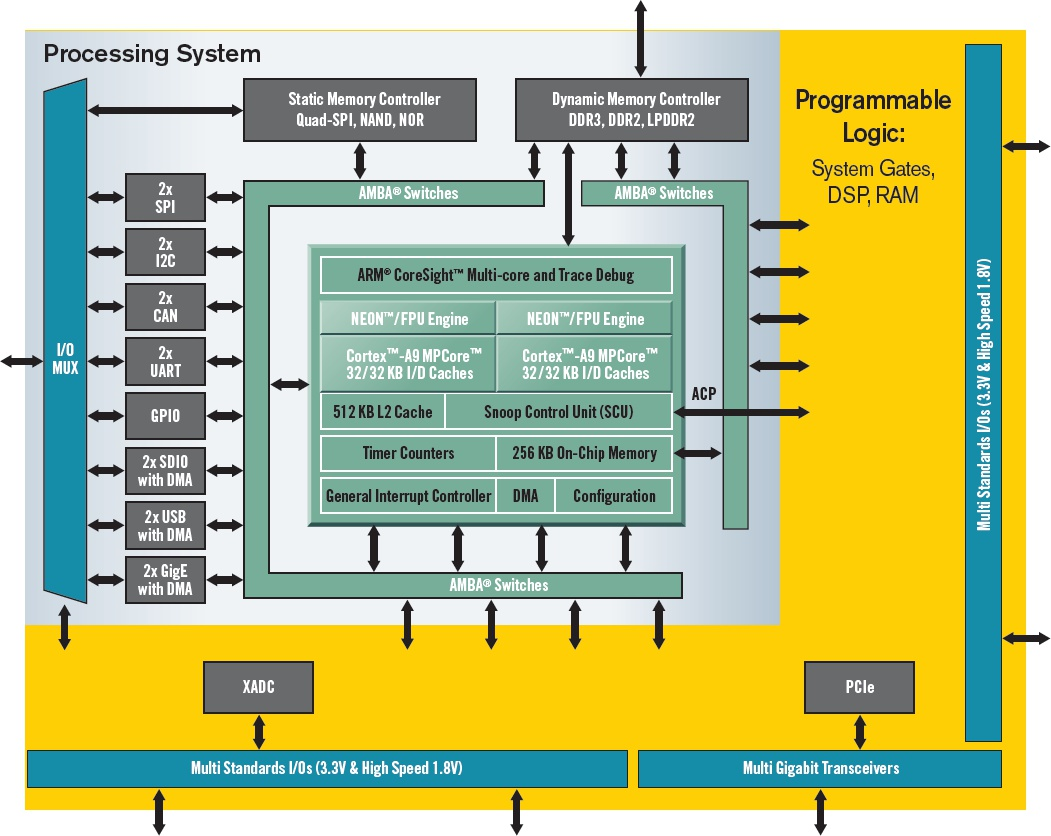
\includegraphics[width=16cm]{img/concept/zynq.png}
%    \caption{Diagram of Zynq SoC~\cite{PIC:ZYNQ_DIAG}}
%    \label{FIG:ZYNQ}
%\end{figure} 
%
%\subsection{Main data transmission interface}
%%TODO Correct style 
%One of the main requirements of the camera framework is the ability to transmit or store acquired video data using a multigigabit
%interface. Among numerous interfaces Serial ATA and Ethernet were chosen as main means of transmitting data.
%These interfaces were chosen because of their high throughput, versatility and maturity. Ethernet currently is becoming 
%more and  more popular in every market, not only for networking applications~\cite{WWW:ETHERCAT}. 
%Serial ATA is widely used in storage devices like Hard Disk Drives and Solid State Drives.
%
%Another key aspect is the way those interfaces can be incorporated into the camera framework. Chosen MPU supports
%multigigabit interfaces using GTP or GTX transceivers, but the design of the IP Core has to be done by the developer,
%which can be time consuming. The easiest approach is to use tested and verified solutions.  
%
%Xilinx provides an IP Core for 1000Base-X Ethernet~\cite{XIL:PCS_PMA} communication, which is supported by Zynq 
%and comes with numerous application notes~\cite{XIL:PG047,XIL:XAPP1082} describing the way of setting up the
%communication. Additionally, it is possible to upgrade the core
%to a 10 GbE version.
%
%On top of this, the camera framework can be easily upgraded to send data through 1 GbE Ethernet or 10 GbE Ethernet using the same SFP
%connector. For the 1 GbE Ethernet to work an IP core is used: Xilinx PCS/PMA 1 GbE IP
%Core~\cite{XIL:PCS_PMA}, which works as a PHY\footnote{Physical layer} for the MAC\footnote{Media Access Controller} 
%incorporated into Zynq SoC~\cite{DSH:TRM}. The pros of this solution, apart from relying on external PHY are presented
%in table\ref{tab:phy}.
%
%%Pros:
%%
%%\begin{itemize}
%%    \item lower cost (1G/10G PHY chips are expensive)
%%    \item more versatile - one can choose 1G or 10GbE depending on application
%%\end{itemize}
%%
%%Cons:
%%\begin{itemize}
%%    \item longer development time 
%%    \item less reliable  
%%\end{itemize}
%%
%\begin{table}
%    \centering
%    \caption{Pros and cons of using an IP based PHY}
%    %\begin{tabular}{|p{3cm}||p{5cm}|p{5cm}|}
%    \begin{tabularx}{\textwidth}{|l|X|X|}
%        \hline
%        & Pros & Cons  \\ 
%        \hline
%        \hline
%        \textbf{Physical PHY}    & 
%        \vspace{0.1cm}
%        \begin{itemize}
%            \item more reliable  
%            \item shorter development time
%        \end{itemize}
%
%        & 
%        \begin{itemize}
%            \item high cost
%            \item fixed solution 
%        \end{itemize}
%
%        \\  
%        \hline
%        \textbf{IP Core PHY}    &  
%
%        \vspace{0.1cm}
%        \begin{itemize}
%            \item lower cost 
%            \item more versatile 
%        \end{itemize}
%
%        & 
%        \begin{itemize}
%            \item longer development time 
%            \item less reliable  
%        \end{itemize}
%
%        \\  
%        \hline
%    \end{tabularx}
%    \label{tab:phy}
%\end{table}
%
%
%
%As for 10GbE, one can use a FADE protocol~\cite{WWW:FADE}. 
%For Serial ATA there is an Open Source IP Core which allows for the data transmission using this interface~\cite{WWW:SATA}.  
%
%\subsubsection{1 GbE with PCS/PMA IP Core}
%1 GbE Ethernet can be used in the framework and the PHY is incorporated via the PCS/PMA IP Core. This idea requires
%the use a SFP transceiver module due to the fact that the transmission is driven directly from the FPGA.  
%
%%  \subsubsection{10 GbE with FADE IP Core}
%%  10 GbE Ethernet can be used in the framework and the PHY is incorporated via the FADE IP Core. This idea requires
%%  to use a SFP transceiver module to work due to the fact that the transmission. 
%
%\subsubsection{Serial ATA}
%The Serial ATA IP Core that is used in this project is available for anyone~\cite{WWW:SATA}. Due to the fact that it
%was designed to be used for Series 6 Xilinx Virtex devices some design changes had to be made. 
%%The clock network was redesigned by mgr inz. Adrian Byszuk. 
%
%%\subsection{Data transfer}
%
%%As for the connectivity the data from the sensor can be send directly via 1 GbE Ethernet using dedicated hardware in 
%%Zynq. This solution provides only 1 Gbps of throughput for the Ethernet, but is very well supported by the 
%%software (drivers are available).
%%
%%I have also tried using SATA interface from Open Cores Repository (opencores.org), but unfortunately this IP core 
%%behaves in a very unstable way and had to be discarded. 
%%
%%The solution that I have chosen, that would provide 10 Gbps of throughput is to use a dedicated FADE protocol IP, 
%%which allows for simple FPGA-PC 10 Gbps Ethernet-based connectivity. This IP core is also available on the opencores. 
%%It was designed by PhD. Wojciech Zabolotny and is extensively used at this moment.  
%%
%%I can only add that PCIe also can be used in this design, but it needs further development.
%%
%%I would like to move further and describe the processing and control. 
%
%
%
%\subsection{Sensor}
%
%%  \subsubsection{CMOSIS (ON Semi) CMV4000} 
%There is a wide variety of sensors available on the market, which might be used in a high speed camera.
%The choice of the sensor must correspond to the most common use of the camera framework. For this project two types of
%sensors were chosen:
%\begin{itemize} 
%    \item standard CMOS sensor - CMOSIS CMV4000\cite{WWW:CMV4000} 
%    \item counting CMOS sensor
%\end{itemize} The different interfaces on both devices allowed for juxtaposing the different methods of interfacing sensors to the 
%Main Processing Unit.
%
%\subsubsection{CMOSIS (ON Semi) CMV4000}~\label{CH3:CMV}
%
%
%The CMV4000\cite{WWW:CMV4000} is a high sensitivity, pipelined global shutter CMOS image sensor with $2048 x 2048$ pixel resolution capable
%of HD format. Pipelining allows exposure during read out. The state-of-the-art pixel architecture offers true correlated
%double sampling (CDS), reducing the fixed pattern noise and dark noise significantly. The imager integrates 16 LVDS
%channels each running at $ 480 Mbps $ resulting in a $ 180 fps $ frame rate at full resolution at 10 bits per pixel. Driving and
%read-out are programmed over a serial peripheral interface. An internal timing generator produces the signals needed for
%read-out and exposure control of the image sensor. External exposure triggering remains possible. A 12 bit per pixel
%mode is available at reduced frame rate.
%
%%
%%Sensor użyty w projekcie to przetwornik video o rozmiarze 1”, wykonany w technologii CMOS. Charakteryzuje się rozdzielczością 2048x2048 punktów i maksymalną szybkością przetwarzania ramek obrazu o wartości 180 klatek/s przy zegarze o częstotliwości 480 MHz (maksymalna częstotliwość zegara dla tego sensora). Sensor posiada 2 wejścia zegarowe – zegar systemowy oraz zegar LVDS. Programowanie rejestrów sensora odbywa się przy pomocy interfejsu SPI. Dane z przetwornika wystawiane są na 16 (lub mniej w zależności od ustawień) wyjść LVDS. Dodatkowo sensor posiada jeszcze 1 wyjście sterujące LVDS, na które wystawiane są sygnały sterujące strumieniem danych oraz 1 wyjście zegara LVDS danych. Dane wystawiane są z częstotliwością równą połowie częstotliwości zegara podanego na wejście zegarowe LVDS na obu zboczach zegara (DDR). Dane na poszczególnych liniach LVDS są wysyłane przez sensor w postaci szeregowej – ze współczynnikiem 10:1 lub 12:1 (w zależności od ustawień przetwornika AC). Wysyłanych jest równolegle 16 serializowanych fragmentów ramki obrazu – po jednym na każde wyjście LVDS. Aby odtworzyć pierwotną postać obrazu, należy najpierw zdeserializować, a następnie przegrupować dane otrzymane od sensora.
%%
%\begin{figure}[h!]
%    \centering
%    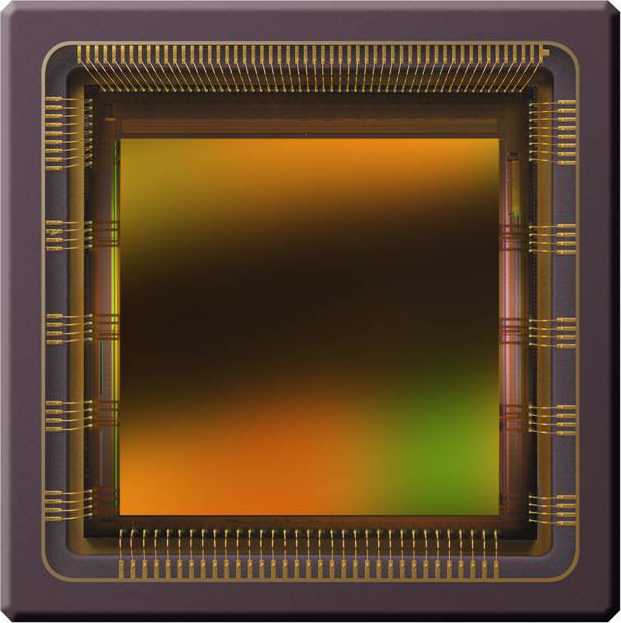
\includegraphics[width=8cm]{img/concept/cmv4000.jpg}
%    \caption{CMV4000 picture\cite{WWW:CMV4000} }
%    \label{fig:CMV4000}
%\end{figure} 
%
%\subsubsection{Counting silicon sensor} 
%In order to properly design the camera framework so that it is flexible in terms of connecting a different sensor,
%an additional device with different architecture has to be used. The camera framework is intended for the use
%in both scientific and commercial markets. Apart from commercial CMOS sensors like CMOSIS CMV4000
%another common type of sensor is CCD or a counting sensor (detector). The first requires the design of a custom Analog
%Front End. This type of design is well described in literature~\cite{MASTER:GK}. For this reason a custom counting
%silicon sensor has been used as a second device. These kinds of sensors are widely used in X-ray imaging and synchrotron
%radiation applications~\cite{WWW:CNT_SENSOR1}. 
%
%The architecture of the readout for this sensor is different from CMOSIS CMV4000, which also adds more in-depth
%information on how it can be implemented in hardware. Data from such a sensor has to be acquired in the form of a continuous stream of data. 
%Physically there is a frame to read, but the architecture is different and more similar to a long shift register, where each pixel
%contains a counter. 
%
%\begin{figure}[h!]
%    \centering
%    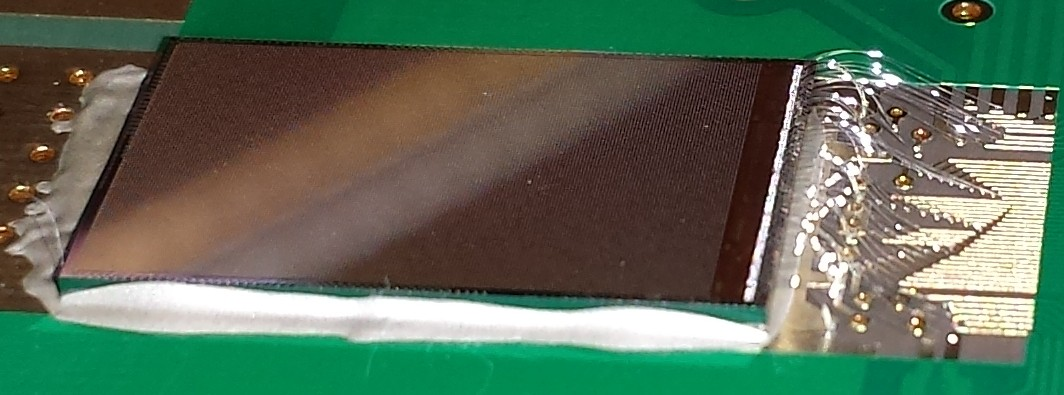
\includegraphics[width=8cm]{img/concept/counting.jpg}
%    \caption{Counting sensor picture\cite{PIC:UFXC}}
%    \label{fig:counting}
%\end{figure} 
%
%
%
%\section{Camera control}
%
%The control of the camera has to be performed over a secure, reliable and high throughput interface. It also should not
%add unnecessary complexity to the design. 
%
%Nowadays, more and more embedded systems are equipped with Ethernet or WLAN so that the communication with the device can
%be performed using a well known TCP/IP protocol. That is why Ethernet was chosen as a main interface for control of the
%camera. Control commands are sent over TCP/IP to the camera in a text format for ease of development. Due to
%security vulnerability, an encryption of the commands can be added as a feature in future versions of the design.
%
%The commands are executed by a Linux socket server, which is the main program running on the OS. The execution of commands
%is done directly by the server application, or by an RTOS. Another key function is the control of the logic fabric through the
%operating system. This is achieved by using a register connected to the main General Purpose AXI bus of Zynq SoC,
%which can be accessed both by operating system and logic fabric.  
%
%%TODO: ADD diagram showing how does the control works
%
% 
%\begin{figure}[h!]
%    \centering
%    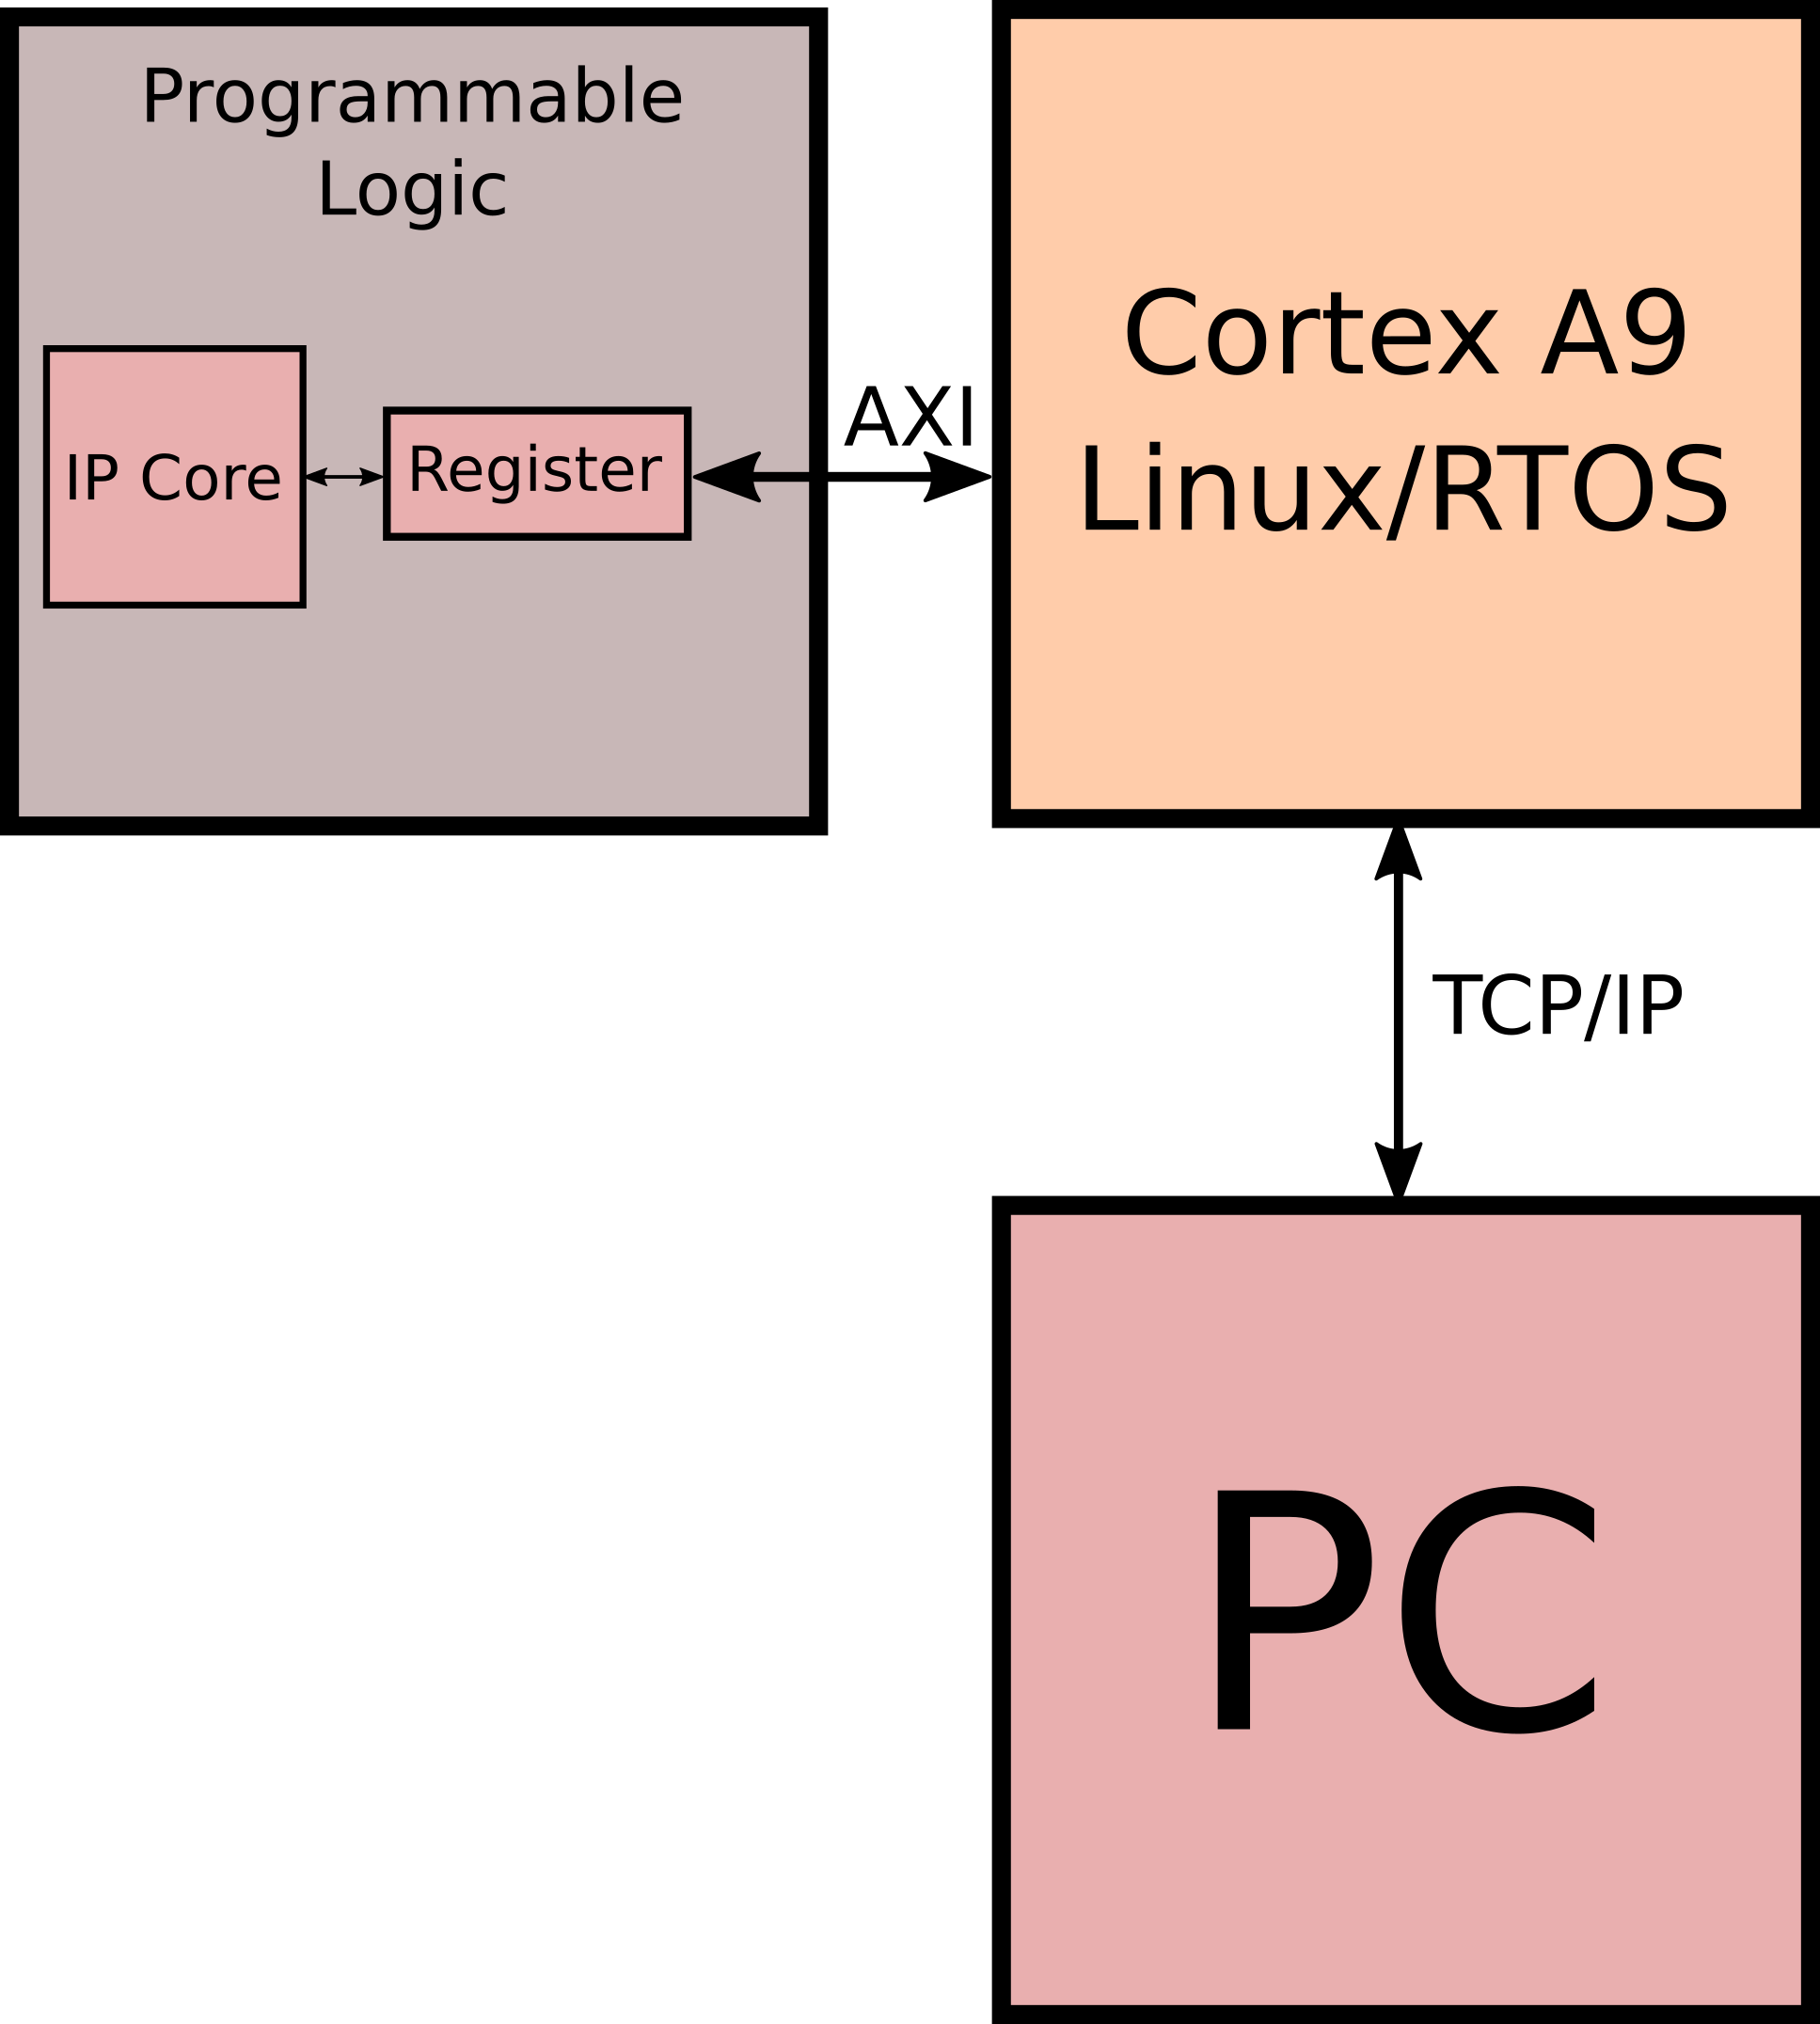
\includegraphics[width=8cm]{img/concept/control_block_diagram.png}
%    \caption{Camera control diagram}
%    \label{FIG:CONTROL_BLOCK_DIAG}
%\end{figure} 
%
%
%
%%\section{Video data processing}
%
%%DMA is responsible for transferring of the data from the sensor to the DDR3 memory and optionally to the 
%%processing system. 
%%
%%This way the data can be buffered in order to send them through dedicated 1 GbE Hardware IP available in Zynq or 
%%e.g. PCIe IP Core given by Xilinx. 
%%
%%In case we want to use a 10 GbE interface there is no need for DMA, because the translation would have to be made. 
%%When 10 GbE interface is needed data are being send directly to this IP Core without the use of DMA.  
%%
%%So at this point we know how are the data acquired form the sensor.
%%
%
%
%%\subsubsection{Serial ATA}
%
%\section{Operating system}\label{ch2:proc_sys}
%
%The operating system is one of the most crucial aspects of any embedded system. The decision of using Zynq SoC with 
%ARM Cortex-A9 which is ARMv7 architecture narrows the possible operating systems that can be run on the processor. 
%ARM Cortex A9 can run baremetal code and many commercial and open source "low-level" operating systems such 
%as: FreeRTOS~\cite{WWW:FREERTOS}, Micrium $\mu$OS~\cite{WWW:MICRIUM}, and GreenHills~\cite{WWW:GREENHILLS}. 
%
%The choice for a specific OS is design dependent. In this thesis, the two most common operating systems were chosen:
%Linux/GNU and FreeRTOS. Both are supported by Xilinx Zynq. Furthermore, three is a way to design an AMP OS where
%on one core there is a Linux and on the other there is FreeRTOS. The communication between Linux OS and RTOS is done by using a
%dedicated \emph{rpmsg} protocol~\cite{XIL:AMP_LINUX_FREERTOS}. 
%
%%As far as processing and control is concerned - Cortex A9 is used for this purpose. Because it's a two core chip, 
%%the designer (that's me) can take advantage of asymmetric multiprocessing. A scenario in which two cores are running 
%%different operating systems in parallel. This approach eases the development, due to the fact that Linux can easily 
%%provide high system level features like TCP/IP stack whereas RTOS is running in a deterministic way and eases the 
%%development of sometimes complex sensor IP control and interrupt handling.
%%
%%Linux is responsible for control of camera operation as well as data processing (optional), and FreeRTOS 
%%is responsible for sensor data acquisition. 
%
%\section{Multichannel operation}\label{ch2:multichannel}
%
%Another key requirement is multichannel operation. In order to provide synchronization between multiple cameras, 
%a PTP (Precision Time Protocol) interface can be used. It is based on Ethernet, which will be available in the design. 
%PTP is widely used by the industry solution which allows for microsecond 
%synchronization. An Open-Source daemon for PTP is evaluated, running on embedded Linux. It allows for synchronisation
%between the cameras in one common Local Area Network. For simple synchronisation, one camera can be a master, whereas
%for more advanced applications a dedicated hardware master with GPS synchronisation should be used.  
%
%
%%Both of this approaches are available in my design, but are not fully implemented and tested. 
%
%%\subsection{PTP}
%
%
%
%%\section{Modelling and desing methodology}~\label{ch2:methodology}
%%
%%  \subsection{Xilinx's Ultra Fast Design Methodology}
%%  
%%  \subsection{Six-Sigma DMAIC}
%%  
%%  \subsection{Waterfall}
%%  
%%  \subsection{Spiral waterfall}
%%  
%%  \subsection{Agile}
%%  
%%  \subsection{UML}
%%  
%%  \subsection{SysML}
%
%\section{Realization methodology}
%%This section presents the approach of the camera framework design. Firstly, the determination of key project decisions
%%a \emph{design process} needs to be planned. 
%%
%%
%%\begin{enumerate}
%%
%%    \item Digital system design - Ethernet and software - hardware control
%%    \item Basic baremetal software for testing of the basic hardware functions
%%    \item Integration of software and hardware
%%    \item Design of Petalinux OS as a main operating system
%%    \item Integration of Petalinux into the hardware subsystem (Control) 
%%
%%\end{enumerate}
%%
%%
%This section presents the realisation phase of the camera framework project, given the requirements set in the 
%concept phase as well as key project decisions. The framework design is very complex, which is why some methodology
%had to be applied in order to successfully realise the project. The key goal of the project is to provide an engineer
%with a basis for development of his own camera system. In order to do so, key design concepts of Zynq
%7 series SoC design methodology are shown first, then the use of those concepts in realizing given functionalities is 
%presented. This way, a reader can both understand the theory and the factual design of the camera framework.
%
%In order to properly design a camera system on Zynq SoC, a certain methodology had to be used. Features and functions
%described in the concept phase were developed one after another, first using a baremetal operating system and, when it was
%ready, it was moved to the camera server application. Baremetal OS allows for direct access to the memory when the cache
%is set specifically so that MMU is not interfering in the operation. 
%
%The methodology can be summed up in the following points:
%
%\begin{itemize}
%
%    \item Develop a feature / function in digital system
%    \item Design a testbench and test the proper operation of digital system IP
%    \item Prepare the control of the IP using AXI Control Register and test it using Baremetal program
%    \item Integrate the control to the OS 
%
%\end{itemize}
%
%
%\section{Project use case}
%This thesis project is meant to be used as a base for a scientific camera design prototype. A designer wishing to use it has
%to choose the required functions and build the system adding needed custom features. Any engineering design has to
%consider how the project will be used before it is realised, so that during development phase it can be done properly. 
%An example of a scientific camera design prototype scenario using the framework is presented below.
%
%The design team needs to verify whether a specific sensor meets the requirements in terms of speed and sensitivity.  
%It might be that a CCD sensor that needs to be cooled to a very low temperature and the mechanical design is extremely
%complicated. Usually, the design would have to be done from scratch even when using off-the-shelf electronics. 
%With the use of the framework, the design team can quickly prototype working electronics acquisition and control system
%for the camera and focus on the design of mechanics (for example). The explanatory process can be arranged in the
%following way:  
%
%\begin{enumerate}
%    \item Design electronics (AFE) to drive the sensor
%    \item Add IP Core for control and use ready digital system for data acquisition from the sensor 
%    \item Modify the control and status information of the system so that it works correctly with the sensor
%    \item Design mechanics with the possibility of using a development board as main electronics
%\end{enumerate}
%
%This is a simplified approach to camera design, but it is obvious that when using the framework, a large
%portion of the work doesn't have to be done for a prototype. This gives a huge advantage to any design team and
%decreases the time-to-market and costs of a scientific design. Obviously there are drawbacks in the form of a fixed type
%of main processing unit (Xilinx Zynq SoC), but in this kind of project the most versatile device has to be used and it
%can be viewed as a temporary solution in a prototype design.   
%
%%The design team can use the framework by adding needed functionality to the project.  a Development Board Xilinx ZC706 and decrease the time to bring
%%the prototype to work.  
%
%%\section{Project team}~\label{ch3:team}
%%This is clearly stated in the sections describing the specific parts. 
%%People who greatly helped me during the development are those mentioned: Grzegorz Kasprowicz, Damian Krystkiewicz,
%%Maciej Trochimiuk, Andrzej Abramowski, Bartłomiej Juszczyk, Adrian Byszuk oraz Krzysztof Sielewicz. 
%
%%For clearance the following modules in the Camera Framework were designed directly by me:
%%\begin{itemize}
%%    \item Petalinux operating system configuration 
%%    \item FreeRTOS implementation on ZC706  
%%    \item modified Serial ATA IP Core in two SSD drive configuration
%%    \item 1000Base-X support with PCS/PMA 
%%    \item Deserialisation of data from silicon counting sensor  
%%    \item baremetal software for digital system control 
%%    \item PTP synchronisation between multiple ZC706 Development Boards
%%    \item system tests
%%\end{itemize}
%%
%
